% CSE 578: Data Visualization - Course Project

\documentclass[journal]{IEEEtran}

% Packages
\usepackage{graphicx}
\usepackage{amsmath}
\usepackage{cite}
\usepackage{placeins}

\begin{document}

% Title
\title{Course Project}

% Author
\author{Andrey Sokolov}

\maketitle

\begin{abstract}
This report presents an in-depth analysis of income-related factors to develop a marketing profile for UVW College. As part of our role at XYZ Data Company, we explored a dataset derived from the US Census Bureau, examining how various demographic and economic attributes influence whether an individual earns more than \$50,000 annually. 

A comprehensive data pipeline was implemented, including data cleaning, feature selection, encoding techniques, and correlation analysis to identify the most impactful variables. Hierarchical clustering and principal component analysis (PCA) were utilized to reduce dimensionality and uncover hidden patterns. Multiple visualization techniques—such as stacked bar charts, heatmaps, and hierarchical clustering dendrograms—were applied to highlight key trends and relationships.

Our findings indicate that factors such as marital status, occupation, education level, and hours worked per week exhibit the strongest correlations with income. Negative correlations with attributes like "relationship" and "sex" suggest structural influences that warrant further exploration. We also compared different classification models, evaluating decision trees, support vector machines (SVM), and neural networks for their predictive accuracy in income classification.

The results of this study will inform UVW College’s enrollment and marketing strategies, allowing for data-driven decision-making. Future work includes refining predictive models, integrating additional socioeconomic data, and developing interactive visual tools to enhance usability for stakeholders.
\end{abstract}

\section{Problem Statement}
In our role as a data analysis firm, our goal is to create a marketing profile for our client, UVW College. We will be exploring the effects of a multitude of factors
on an individual's income and in particular, whether they can be used to help determine whether an individual earns more than 50,000 USD per year. XYZ company will analyze
variables such as education, occupation, and marital status - sourced from the US Census Bureau - to be used in the creation of visualizations to help us create a marketing profile and a predictive model for the college. These will guide
UVW College in its marketing and enrollment campaign strategies.


\section{Work Completed So Far}

\subsection{Background Tasks Completed}
\begin{enumerate}
    \item Latex set up for drafting submissions in VS Code for Mac by installing Mactex
    \item Started a Jupyter notebook server and began coding/using markdown to explain each data analysis step
    \item Installed and configured necessary Python libraries, including: 
    \texttt{pandas}, \texttt{seaborn}, \texttt{matplotlib}, and 
    \texttt{scikit-learn}.
    \item Set up Git version control to track code changes and manage different analysis iterations.
    \item Started a Jupyter notebook server and began coding and markdown to explain each data analysis step
    \item Documented key findings and insights in Jupyter notebooks for reference in the final report.
\end{enumerate}

\subsection{Data Cleaning Approach}
One of the initial challenges was ensuring the dataset was clean and structured correctly. The dataset contained missing values, inconsistencies in categorical variables, and redundant features. The steps taken were:
\begin{itemize}
    \item Removed 'fnlwgt' from DataFrame as it will not be used
    \item Identified and removed leading/trailing whitespace characters in multiple columns, identified by isolating unique values
    \item Checked for minimum and maximum of all continuous variables as well as any negative values. There are two maximums that seem to be capped - capital-gain(99999) and hours-per-week(99)
    \item Also identified missing values in the data, marked as '?'. These were replaced with 'None' as an indicator of missing values for Python interpretation
    \item Noted - number of missing values is quite low and only for a few variables - workclass and occuption(a correlated number) and native-country
\end{itemize}

\section{Challenges and Solutions}

\subsection{Issues Encountered and Solutions}

\begin{description}
    \item[Q:] \textbf{Which attributes should be prioritized for analysis? How should they be chosen?}
    \item[A:] Initially, attribute selection was based on intuition and cursory data exploration. However, to ensure an evidence-based approach, correlation analysis and feature importance techniques should be applied. Attributes with strong correlations to income can be refined from preliminary machine learning models or manual EDA.

    \item[Q:] \textbf{What is the best algorithm to classify/model this kind of data? Decision Tree vs. SVM vs. Neural Network?}
    \item[A:] Several machine learning algorithms were considered and researched. A Decision Tree model seems like a good fit because it offers interpretability and handles categorical data well.

\end{description}

\subsection{Remaining Tasks and Approach}
\begin{description}
    \item[Q:] \textbf{What tasks remain to be completed?}
    \item[A:] The following tasks are pending:
    \begin{itemize}
        \item Prioritizing attributes,following requirements for minimums and different chart types
        \item Craft/finalize user stories, one for the current visualization and at least four more
        \item Conduct deeper analysis on interaction effects between multiple factors.
        \item Verify insights against real-world expectations and research findings.
        \item Assess effectiveness of different machine learning models for classification.
        \item Writing the final report with conclusions based on insights derived from visualizations and models.
    \end{itemize}

    \item[Q:] \textbf{How will these tasks be approached?}
    \item[A:] 
    \begin{itemize}
        \item Use additional statistical validation to confirm feature relevance.
        \item Review to ensure that visualizations are aligned with project objectives and meet stated goals.
        \item Prepare structured documentation summarizing findings, methodology, and business implications for UVW College.
    \end{itemize}
\end{description}


\subsection{Choosing the First Attributes for Analysis}
The first step in feature selection was identifying the most relevant attributes affecting income classification. The following approach was taken:
\begin{itemize}
    \item Conducted an initial exploratory data analysis to find at least one predictive attribute
    \item Selected \textbf{Education} as the primary attribute for early investigation, as it showed promising correlation with income level.
\end{itemize}

\subsection{Creating the First Visualization}
To validate early assumptions, the first visualization was created:
\begin{itemize}
    \item To plot salary versus education, we considered the binary nature of our key factor, salary. Since it is broken up into less than 50K and greater than 50K, it makes sense to plot using another attribute as an axis.
    \item Education is already broken up into integer values in the education-num category, but there are too many categories to comfortably display
    \item Therefore, we can consolidate the grade levels into one block, the non high school grad - this reduces down to 8 educational categories.
    \item Some thought was given to keeping associate degree (vocational) as "trade school", but outcomes are so similar to the traditional associate degree that it made more sense to combine the two
    \item Design Choices: Used distinct color coding for income categories, clear axis labeling, and a balanced layout for readability.
    \item Implementation: The visualization was created using Seaborn in Python.
    \item The aggregate visualization did a good job at representing the correlation between each education bracket and salary, but clarity was further improved by sorting by education level left to right
\end{itemize}

\begin{figure}[h]
    \centering
    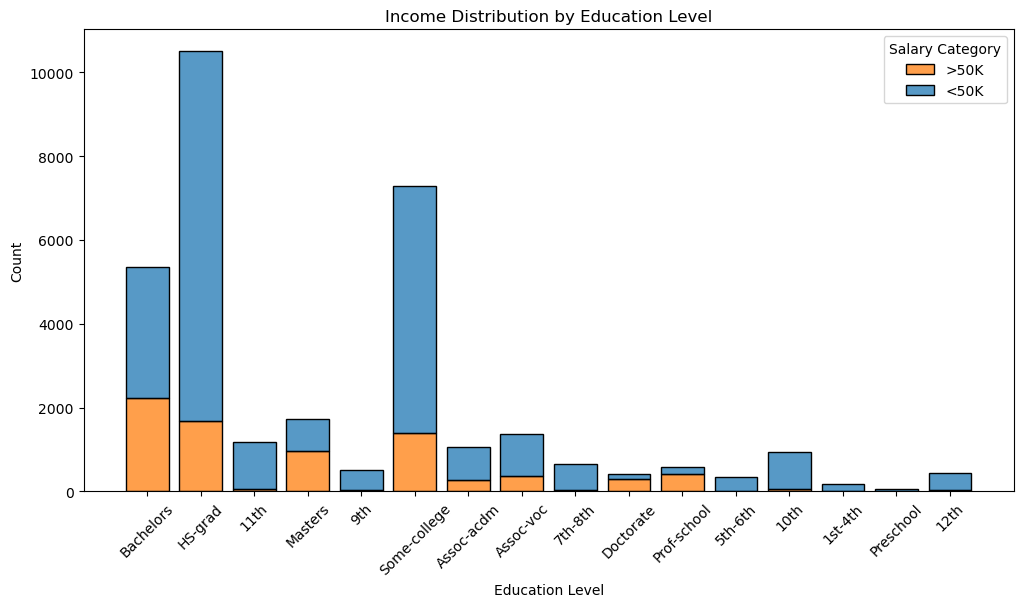
\includegraphics[width=\columnwidth]{hist_bad.png}  % Fit within one column
    \caption{Income vs Education without aggregates and ranked order}
    \label{fig:Income vs Education without aggregates and order}
\end{figure}

\begin{figure}[h]
    \centering
    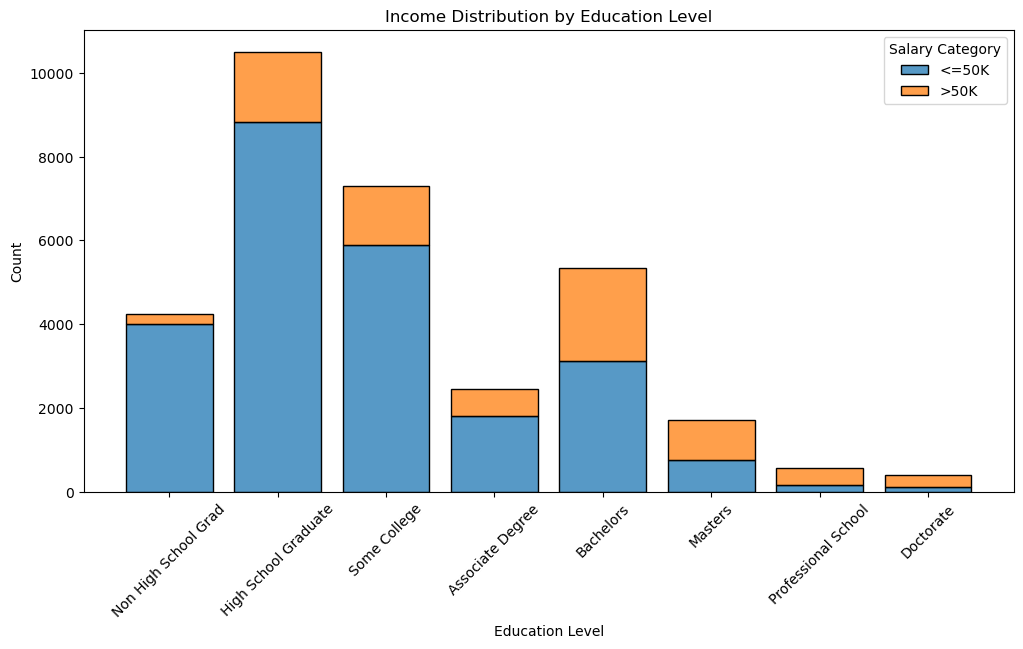
\includegraphics[width=\columnwidth]{hist_4.png}  % Fit within one column
    \caption{Final histogram for Income vs Education}
    \label{fig:Final histogram for Income vs Education}
\end{figure}

\section{Initial / Key Insights from Education Level vs. Income Distribution}

\begin{itemize}
    \item \textbf{Higher Education Correlates with Higher Income:} Individuals with advanced degrees (Masters, Professional School, Doctorate) have a significantly higher proportion of incomes above \$50K compared to those with lower educational attainment.
    
    \item \textbf{Most Common Education Levels:} The majority of individuals fall into the \textit{High School Graduate} and \textit{Some College} categories, making them the largest groups in the dataset. However, their income distributions do not show their education to be a predictor for the less than \$50K and greater than \$50K groups.
    
    \item \textbf{Education Alone is Not a Sole Predictor of Income:} Even at the Bachelor's level, a substantial number of individuals still earn less than \$50K. This suggests that additional factors such as work class, occupation, and experience must be considered to better predict income.
\end{itemize}


\section{Tentative User Stories}
To structure our approach, we defined the following user stories that represent key stakeholders:

\subsection{User Story \#1}
\begin{itemize}
    \item \textbf{Role:} Analyst at UVW marketing team
    \item \textbf{Goal:} To determine if education level significantly impacts income classification.
\end{itemize}

\subsection{User Story \#2}
\begin{itemize}
    \item \textbf{Role:} Director of the UVW marketing team
    \item \textbf{Goal:} To analyze how the combination of occupation type, hours worked per week, and capital gains influences salary category.
\end{itemize}

\subsection{User Story \#3}
\begin{itemize}
    \item \textbf{Role:} Workforce development strategist
    \item \textbf{Goal:} To examine variations in income levels across different work classes and education levels.
\end{itemize}

\subsection{User Story \#4}
\begin{itemize}
    \item \textbf{Role:} Director of the UVW marketing team
    \item \textbf{Goal:} To identify the strongest predictors of high-income individuals.
\end{itemize}

\subsection{User Story \#5}
\begin{itemize}
    \item \textbf{Role:} UVW Policy analyst
    \item \textbf{Goal:} To assess whether marital status plays a significant role in salary levels across different age groups.
\end{itemize}

\subsection{User Story \#6}
\begin{itemize}
    \item \textbf{Role:} UVW Foreign relations researcher
    \item \textbf{Goal:} To compare income variations among individuals based on their native country and work class.
\end{itemize}


\section{Python Code Todo}
Submit the Python code as a separate PDF with appropriate documentation and comments for clarity.

\end{document}
